\chapter{Bend Geometry in Liquid Crystals}
\label{ch:TwistBend}
\section{The structure of bend zeros}
\begin{figure}[htbp]
    \centering
    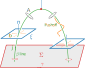
\includegraphics[keepaspectration, width=0.7\linewidth ]{\TwistBendFigures/BetaLine6.pdf}
    \caption{hi}
    \label{fig:BetaLines}
\end{figure}

Consider the 1-form $B := \langle b,b \rangle A$ and its dual vector $\w{B} := \langle B, \bullet \rangle$. The vector $\mathbf{j} := \nabla \times \mathbf{B}$ points along the $\beta$ lines, orienting them according to the circulation of $A$ as shown in figure~\ref{fig:BetaLines} \cite{Machon2016b}. To see this, consider a local trivialisation $(\w d_x, \w d_y,\w n)$ in a tubular neighbourhood around the $\beta$ line. Unlike $(\mathbf{b}, \mathbf{b}_\perp)$, $(\w d_x, \w d_y)$ are nonzero throughout the neighbourhood. In such a trivialisation, ${\bf b} = b_x \w{d}_x + b_y \w{d}_y,\ {\bf b}_\perp = b_x \w{d}_y - b_y \w{d}_x,\ \langle \w b, \w{b} \rangle = b_x^2 + b_y^2$. Expanding $A$ one finds
\begin{equation}
    A = \frac{b_x d b_y - b_y d b_x}{b_x^2 + b_y^2}+ \omega
    \label{eq:localA}
\end{equation}
where \omega := $\langle \w{d}_y, \nabla \w{d}_x \rangle$ is the connection $1$-form associated to $\nabla$ when using this local trivialisation. $(b_x,b_y,s)$, where $s$ is arclength along the $\beta$ line, form a local coordinate system with $z$-axis tangent to the $\beta$ line and given by $\nabla b_x \times \nabla b_y/|\nabla b_x \times \nabla b_y|$ --- generically $(b_x, b_y)$ vanish linearly, so $\nabla b_x, \nabla b_y$ are non-zero on the $\beta$ line and the coordinate system is well defined. We may also define the associated cylindrical polar system $(\rho,\theta,z)$\footnote{Always remember, however, that the vectors $\nabla b_x/|\nabla b_x|$ and $\nabla b_y/|\nabla b_y|$ are not orthogonal and so there is a Jacobian between this and a `true' polar system.}, in which $A = d\theta + \omega$. The azimuthal 1-form $d\theta$ itself is undefined on the $\beta$ line, diverging relative to the smooth contribution $\omega$, and as such the essential behaviour of $A$ around the $\beta$ line is simply that of $d \theta$ (figure~\ref{fig:BetaLines}). Multiplying \eqref{eq:localA} through by $b_x^2 + b_y^2$, $\w{B} = b_x \nabla b_y - b_y \nabla b_x + (b_x^2 + b_y^2) \langle \omega, \bullet \rangle$  and on the $\beta$ line $\w{j} = \nabla \times \w{B} = 2 \nabla b_x \times \nabla b_y$. In terms of differential forms, on the $\beta$ line $dB = 2 d b_x \wedge d b_y$ and $\star dB$ is dual to $\w j$, where $\star$ denotes Hodge duality. We emphasise that $A$ and $d\theta$ are defined along the entire tubular neighborhood of a generic $\beta$ line (with the line itself cut out), providing a canonical orientation.

\subsection{The local structure of bend zeros}
We may investigate the local structure of a $\beta$ line via a Taylor series in $\w b$. Genercially this is governed by linear terms, and so this is equivalent to examining the structure of $\nabla \w b$ on the $\beta$ line. We have already seen that the director $\w n$ splits $T \mathbb{R}^3\approx L \oplus \xi$, with a corresponding splitting of $\nabla \w n$ into two pieces, $\nabla^L \w n $ and $\nabla^\xi \w n$, in \S\ref{subsec:Geometry}, and one way to proceed is to do same to $\nabla \w b$. However, the $\beta$ line itself, in combination with $\w n$ along it, provides us with more structure than a single splitting --- it gives a canonical way to further split $\xi$, giving an adapated framing with which several other planes and splittings may then be defined. In figure \ref{fig:Splittings}(a) we show the $\beta$ line and $\w n$ at a generic point, where $\w n$ and $\w j$ are neither parallel nor perpendicular. The normalised cross product $\w n \times \w j$ defines a vector $\w n_\lambda := \w n \times \w j/| \w n \times \w j|$ and orthogonal plane $\lambda$, and we define a third vector $\w n_\chi := \w n_\lambda \times \w n = (\w j - (\w n\cdot \w j)\w n)/|\w j - (\w n\cdot \w j)\w n|$, the normalised projection of $\w j$ onto $\xi$, with associated orthogonal plane $\chi$. Setting $(\w d_x, \w d_y, \w n) = (\w n_\chi, \w n_\lambda, \w n)$ gives an adapted frame for the $\beta$ line, with the line itself always in the $\lambda$ plane. Note immeadiately that by construction, $\w n_\chi \cdot \w j \geq 0$, and further that this frame is undefined if $\w n \parallel \w j$. Across such points both $\w n_\chi$ and $\w n_\lambda$ change sign discontinuously, and the framing undergoes a $\pi$ rotation (as unoriented planes $\chi$ and $\lambda$ may be extended by continuity) --- this situtation is shown in figure  \ref{fig:Splittings}(b), and we shall return to it in a moment. As well as $\xi, \chi$ and $\lambda$, we also have the plane perpendicular to $\w j$ itself, given by $\mathrm{ker}(\star dB)$ and denoted $\alpha$. Loops in these planes measure winding about the $\beta$ line. We have two limiting cases, shown in figures \ref{fig:Splittings}(b) and (c). In figure~\ref{fig:Splittings}(b), $\w  n \parallel \w j$, $\xi = \alpha$ and a loop in $\chi$ intersects the $\beta$ line --- if we try to measure winding on this plane we encounter degenerate behaviour. In figure~\ref{fig:Splittings}(c) $\w n \perp \w j$, $\chi = \alpha$ and a loop in $\xi$  intersects the $\beta$ line, likewise showing degenerate behaviour. This latter case, where $\w n \cdot \w j= 0$, we refer to as a Legendrian point \citep{Geiges2009}. One notes that the degeneracy in figure \ref{fig:Splittings}(b) is of higher codimension than that in \ref{fig:Splittings}(c).
\begin{figure}[htbp]
    \centering
    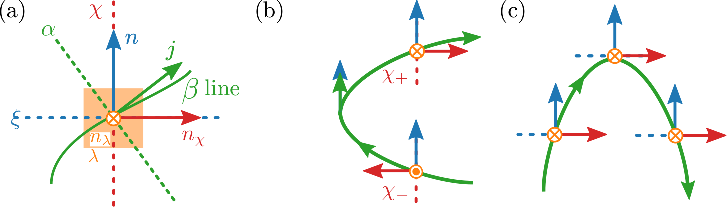
\includegraphics[keepaspectration, width=0.99\linewidth ]{\TwistBendFigures/Splittings.pdf}
    \caption{hi}
    \label{fig:Splittings}
\end{figure}

We now examine the structure of $\nabla \w b$ on the $\beta$ line, making use of the various planes defined above. In general, $\nabla \w b \in \Gamma(T^*\mathbb{R}^3 \otimes T\mathbb{R}^3)$. Note, however, that $\langle \w n, \nabla \w b \rangle = - \langle \w b , \nabla \w n \rangle$ and so along a $\beta$ line, where $\w b=0$, $\nabla \w b$ takes values in $T^*\mathbb{R}^3 \otimes \xi$ and so can be viwed as a linear map $\mathbb{R}^3 \rightarrow \mathbb{R}^2$, with a one-dimensional kernel which defines the $\beta$ line; $\w j$ lies in this kernel. We have that 
\begin{equation}
    \w j = \mathrm{det}(\nabla^{\alpha} \w b) \hat{\w j} = \mathrm{det}(\nabla^\xi \w b) \w n + \mathrm{det}(\nabla^\chi \w b) \w n_\chi
\label{eq:IndexRelation}
\end{equation}
where, as defined in \s{\ref{subsec:Geometry}}, $\nabla^\bullet \w b$ is the restriction of $\nabla \w b \in \Gamma(T^*\mathbb{R}^3 \otimes \xi) $ to the space $\bullet^* \otimes \xi$. It is understood that each $\nabla^\bullet \w b$ is evaluated on the $\beta$ line, and one may imagine each reads $\nabla^\bullet \w b |_{\beta\ \mathrm{line}}$ although we shall not explicitly write the evaluation. Each equality in \eqref{eq:IndexRelation} is just a rewriting of the cross product $\nabla b_x \times \nabla b_y$, but they may be obtained directly by pulling back the volume form on $\xi$ via $\nabla \w b$. Using the second equality  in \eqref{eq:IndexRelation} as an example, we have the decomposition $\nabla \w b = \nabla^\xi \w b E_\xi + \nabla^\chi \w b E_\chi+ \nabla^\lambda \w b E_\lambda$, where $E_\bullet$ denotes projection onto the subspace $\bullet$ as in \s{\ref{subsec:Geometry}. This decomposition carries through to the pullback, and since each of $\nabla^\xi \w b , \nabla^\chi \w b,\nabla^\lambda \w b $ is a map between vector spaces of the same dimension, the pullback simply scales the volume form by the determinant. Finally, by the construction of our framing, $\mathrm{det}(\nabla^\lambda \w b) =0$ --- if we were using an arbitrary framing all three terms would appear in \eqref{eq:IndexRelation}. Recall also that, by the construction of $\w n_\chi$, $\det\nabla^\chi \w b \geq 0$.

 \eqref{eq:IndexRelation} relates the windings we see in different measuring loops around the $\beta$ line, and allows us to examine winding behaviour as we pass through a Legendrian point. In the above discussion we focused on $\xi$ and $\chi$, but it is worth also describing what one observes when measuring winding on a general oriented plane $\gamma$. Pairing a unit vector in $\mathbb{R}^3$ to its orthogonal oriented plane, the space of all such planes is $S^2$, and we imagine $\w j $ defining a north pole. The set of all planes containing the $\beta$ line is then an equatorial circle which splits $S^2$ into two disconnected hemispheres --- in passing from one piece to another we encounter a plane containing the $\beta$ line, on which $\mathrm{det}(\nabla^\gamma \w b) = 0$ and across which it changes sign. This description motivates the definition of an index $ I^\gamma_\beta := \mathrm{Sgn}(\mathrm{det}(\nabla^\gamma \w b)) =\mathrm{Sgn}(\w n_\gamma \cdot \w j)$, where $\w n_\gamma$ is the unit vector associated with the oriented plane $\gamma$. The most common measurement of this type is $I^\xi_\beta$ \citep{Nye1987,Berry1998,Berry2004}, which describes the winding of $\w b$ measured on a loop in the oriented plane $\xi$. The value of $I^\gamma_\beta$ depends on which of the two equivalence classes outlined above $\gamma$ belongs to; if $\gamma$ is degenerate and $\mathrm{det}(\nabla^\gamma \w b)=0$, we set $I^\gamma_\beta=0$. By construction, $I^\lambda_\beta=0$, $I^\chi_\beta= \{0,1\}$. This latter fact is a little subtle given the reversal of $\w n_\chi$ when $\w n \parallel \w j$; we return to it in a moment.  

 Let us now consider situations of degeneracy in order of ascending codimension, beginning with a Legendrian point, shown in figure~\ref{fig:Splittings}(c). At the point itself $\w n \cdot \w j =0$ so $I^\xi_\beta=0$ and we encounter degenerate winding on $\xi$; across the point $I^\xi_\beta$ changes sign. By contrast, the winding measured in $\alpha = \chi$, given by $I^{\chi}_\beta$, is perfectly well behaved. The dual situation, of higher codimension, occurs when $\w n \cdot \w j = \pm 1$, $I^\chi_\beta=0$ and is shown in figure \ref{fig:Splittings}(b). Across such points, the orientation of $\chi$ reverses. To be precise let us define a $+$ and $-$ side of the point, with associated oriented planes $\chi_+$ and $\chi_-$ which may be smoothly continued across the singular point and so defined on a neighborhood of it. On the $+$ side $I^\chi_\beta = I_\beta^{\chi_+}$, and on the $-$ side $I_{\beta}^\chi = I_{\beta}^{\chi_-}$. We have that $I_{\beta}^{\chi_+} = -I_{\beta}^{\chi_-}$ and so measurement of index on a consistently oriented plane across the singular point shows a sign reversal. Finally $\mathrm{det}(\nabla^{\alpha}\w b)^2 = \mathrm{det}(\nabla^\xi \w b)^2+ \mathrm{det}(\nabla^\chi \w b)^2$, and so for $I^{\mathrm{\alpha}}_\beta$ to vanish we require that $I^\xi_\beta = I^\chi_\beta = I^\lambda_\beta=0$, in other words that $\w j$ vanish, an even higher codimension degeneracy in which $\mathrm{ker}(\nabla \w b)$ become two-dimensional and the coordinate system $(b_x,b_y)$ defined above breaks down. 

We briefly explore how these constructions appear when given a concrete, but arbitary, trivialisation $(\w d_x,\w d_y,\w n)$. With respect to this trivialisation $\nabla \w b$ is given a $2\times3$ matrix and we have a Taylor series
\begin{align}
\begin{pmatrix}b_x \\ b_y\end{pmatrix} = 
\begin{pmatrix} 
    \nabla^\xi \w b_{xx} & \nabla^\xi \w b_{xy} & s_{xz}\\
    \nabla^\xi \w b_{yx} & \nabla^\xi \w b_{yy} & s_{yz}\\ 
\end{pmatrix}
\begin{pmatrix}x \\ y \\ z \end{pmatrix}  
+ O(2)
\label{eq:gradbmatrix}
\end{align}
where $s_{xz},s_{yz}$ are currently regarded simply as undetermined constants in the Taylor series. How should we extract the adapted frame, orientation of the $\beta$ line and local windings from this matrix? $I_\beta^\xi$ is immediate. $\w j$ is given by
\begin{align}
    \w j &= (\nabla^\xi \w b_{xy}s_{yz} - \nabla^\xi \w b_{yy}s_{xz})\w d_x -( \nabla^\xi \w b_{xx}s_{yz} - \nabla^\xi \w b_{yx}s_{xz})\w d_y + \mathrm{det}(\nabla^\xi \w b) \w n \\
         &= \mathrm{det}(\nabla^{\chi^{'}} \w b)\w d_x  -\mathrm{det}(\nabla^{\lambda^{'}} \w b)\w d_y + \mathrm{det}(\nabla^\xi \w b) \w n = \mathrm{det}(\nabla^{\chi}\w b)\w n_\chi + \mathrm{det}(\nabla^\xi \w b) \w n
\end{align}
where $\chi'$ and $\lambda'$ are the planes associated to the unadapted frame $(\w d_x,\w d_y, \w n)$. We have that $\mathrm{det}(\nabla^{\chi} \w b)= (\mathrm{det}(\nabla^{\lambda^{'}} \w b)^2 + \mathrm{det}(\nabla^{\chi'}\w b)^2)^\frac{1}{2}$, where we may safely choose the positive branch of the square root by construction of $\w n_\chi$. Away from a Legendrian point $\w{j}$ may also be written as $\w j = \mathrm{det}(\nabla^\xi \w b)(\nabla^\xi \w b^{-1}\w{s},1)^T$, where $\w s = (s_{xz}, s_{yz})^T$, and so the orientation on the $\beta$ line is determined by $\nabla^\xi \w b^{-1} \w s$ --- specifically, its angle to the local $z$-axis is given by $\tan\theta = \mathrm{det}(\nabla^{\chi}\w b)/ \mathrm{det}(\nabla^{\xi}\w b)= \w s^T (\nabla^\xi \w b^{-1})^T \nabla^\xi \w b^{-1} \w s$, and to the $x$-axis by $\cos \phi =\mathrm{det}(\nabla^{\chi'}\w b) /\mathrm{det}(\nabla^{\chi}\w b)$ --- a rotation by $\phi$ adapts the framing, bringing $\chi'=\chi, \lambda' = \lambda$, at which point \eqref{eq:gradbmatrix} adopts the form
\begin{align}
\begin{pmatrix}b_x \\ b_y\end{pmatrix} = 
\begin{pmatrix} 
     \cot \theta s_{xz}& \nabla^\xi \w b_{xy} &s_{xz}\\
    \cot \theta s_{yz}& \nabla^\xi \w b_{yy} & s_{yz}\\ 
\end{pmatrix}
\begin{pmatrix}x \\ y \\ z \end{pmatrix}  
+O(2)
\label{eq:gradbmatrix}
\end{align}
where $\nabla^\xi \w b_{xy}$ etc. now refer to the rotated coordinate values. At a Legendrian point, $\mathrm{det}(\nabla^\xi \w b)=0$, but \eqref{eq:gradbmatrix} and our expression for $\cos \phi$ still hold in the limit $\theta \rightarrow \pi/2, \cot \theta \rightarrow 0$. The limit where $\theta \rightarrow 0$ is a little more delicate. Here $s_{xz}, s_{yz} \rightarrow 0$, and one needs to prescribe a manner in which they do so in order to find the limiting framing behaviour --- for example, $\cos\phi = (1+(\mathrm{det}\nabla^\lambda' \w b)^2 /(\mathrm{det}\nabla^\lambda' \w b)^2)^{-\frac{1}{2}} = (1+ (\nabla^\xi \w b_{xx} s_{xz} - \nabla^\xi \w b_{yx} s_{yz})^2/(\nabla^\xi \w b_{yx}s_{xz}-\nabla^\xi \w b_{yy} s_{yz})^2)^{-\frac{1}{2}}$, and this expression can give arbitary values of $\phi$ depending on how the limits in $s_{xz}, s_{yz}$ occur.
\subsection{Relating $\beta$ line structure to director gradients}
 Above, we studied the structure of $\nabla \w b$ on $\beta$ lines and the possible local structures of bend around them. All of this structure is derived from that of $\w n$, and it is interesting to investigate their correspondence. For example, it is relatively easy to imagine a director field which gives a bend zero with index $I^\xi_\beta=+1$: we picture $\w n$ tangent to a family of helices all centered on a local axis, their radius decreasing as one approaches the axis and degenerating a line along the axis itself. A director with $I^\xi_\beta=-1$ is perhaps less obvious; how should we construct and visualise one? 

We begin by relating bend structure about a $\beta$ line to director gradients: a direct calculation yields $\nabla^\xi \w{b} = (\nabla^\xi{\bf n})^2+\nabla^L \nabla^\xi{\bf n}$ , $\nabla^L \w b = (\nabla^L)^2 \w n$. With respect to an arbitrary $(\w d_x,\w d_y, \w n)$ trivialisation the corresponding Taylor series for the director, retaining only terms that contribute to the bend at linear order, is
\begin{align}
\begin{pmatrix} n_x \\ n_y \end{pmatrix} & = \biggl( \nabla^\xi {\bf n}  + z  \nabla^L\nabla^\xi {\bf n} \biggr) \begin{pmatrix} x \\ y \end{pmatrix} + \frac{1}{2} z^2 \begin{pmatrix} (\nabla^L)^2 n_x \\ (\nabla^L)^2 n_y \end{pmatrix} \\
\label{eq:DirectorTaylor}
\end{align}
giving bend
\begin{align}
\begin{pmatrix}b_x \\ b_y\end{pmatrix} & =
\biggl(\left(\nabla^\xi {\bf n}\right)^2+ \nabla^L\nabla^\xi {\bf n} \biggr) \begin{pmatrix} x \\ y \end{pmatrix}
 + z \begin{pmatrix}(\nabla^L)^2 n_x \\ (\nabla^L)^2 n_y \end{pmatrix},,,,
\label{eq:BendTaylor}
\end{align}
which may then be cast into the form of \eqref{eq:gradbmatrix}. We emphasise again that all operators in \eqref{eq:DirectorTaylor}, \eqref{eq:BendTaylor} are evaluted on the $\beta$ line. Pursuing our investigation of zeros of differing index we decompose $\nabla^\xi \w{b}$ into two components, a spin 0 component $\nabla^{\xi, +} \w{b}$ with positive determinant and winding, and a spin 2 component $\nabla^{\xi, -} \w{b}$ with negative determinant and winding: $\nabla^\xi \w{b} = \nabla^{\xi,+} \w{b} + \nabla^{\xi,-} \w{b}$. With this decomposition one finds that $\w{n} \cdot \w{j} = \mathrm{det}(\nabla^\xi \w{b}) = |\mathrm{det}(\nabla^{\xi, +} \w{b})| - |\mathrm{det}(\nabla^{\xi, -} \w{b})| $ and so the relative weights of each component determine the overall index. $\nabla^{\xi,+} \w{b}$, $\nabla^{\xi,-} \w{b}$ may again be explicitly computed in terms of the director by recalling the splitting of the shape operator~\eqref{eq:GradientDecompositionperp}
\begin{align}
    \nabla^\xi {\bf n}= \frac{\nabla \cdot {\bf n}}{2}I_\xi + \frac{{\bf n} \cdot \nabla \times {\bf n}}{2} J + \Delta
\end{align} 
which, with respect to our local $(\w d_1,\w d_2,\w n)$ basis, reads 
\begin{align}
 \nabla^\xi {\bf n}=\begin{pmatrix} s/2 + \Delta_1 & -q/2 + \Delta_2 \\ q/2 + \Delta_2 & s/2 - \Delta_1 \end{pmatrix}
\end{align} 
where $s = \nabla \cdot \w n$ is the splay, $q = \w n \cdot \nabla \times \w n$ is the twist and $\Delta_1$, $\Delta_2$ are the deviatoric components~\citep{Machon2016b,AlexanderBook,Selinger2019}, all evaluated on the $\beta$ line. We find that
\begin{align}
\nabla^{\xi,+} \w{b} &=
\frac{1}{4}\Big(s^2 - q^2 + 4\Delta_1^2 + 4\Delta_2^2 +2\nabla^L s\Big)I_\xi+
\frac{1}{2} \Big(sq + \nabla^L q \Big)J,  \\
\nabla^{\xi,-} \w{b} &= s \Delta +\nabla^L \Delta.
\end{align}
 Note that in the absence of variation along $\w n$, $\nabla^\xi \w{b} = (\nabla^\xi{\bf n})^2$ and only an index of $I^\xi_\beta = +1$ is possible. The potential for negative winding is thus entirely contained within $\nabla^L \Delta$. Explicitly, $\w{n} \cdot \w{j} = \mathrm{det}(\nabla^\xi \w{b}) = \left( (s/2)^2 +(q/2)^2 -\Delta_1^2 - \Delta_2^2\right)^2 +\left(s(q/2)^2 + \nabla^L (q/2)\right)^2 - (\nabla^L \Delta_1) ^2 - (\nabla^L \Delta_2)^2 - s \nabla^L(\Delta_1^2 + \Delta_2^2)$.  In figure \ref{fig:LocalProfiles} we show a variety of bend zeros with indices $I^\xi_\beta = \pm 1$ and their accompanying modes of director distortion.

\begin{figure}[htbp]
    \centering
    \includegraphics[keepaspectration, width=0.7\linewidth ]{\TwistBendFigures/LocalProfiles.pdf}
    \caption{Local profiles about $I_\beta = +1$ (green line) and $I_\beta = -1$ (red line) bend zeros, with director (blue cylinders) and bend vector (orange) shown in cross-section. Each panel shows the effect of a single parameter in  with the rest set to zero. $z$ variation in $\Delta$ is essential for a $I_\beta = -1$ zero.}
    \label{fig:LocalProfiles}
\end{figure}


\begin{comment}







\section{Topological Significance}

On the complement of the bend zeros, we define an orthonormal connection 1-form
\begin{equation}
    A = \langle \nabla \tilde{e}_1 ,\tilde{e}_2 \rangle = \frac{\langle \nabla e_1 ,e_2 \rangle}{\langle e_1,e_1 \rangle}  
\end{equation}

where $\tilde{e}_i$ is the normalised version of $e_i$. A few remarks about this definition are in order. Firstly, the connecction $\nabla$ at play here is a connection on the bundle $\xi$, and is globally well defined as the restriction of the ambient connection of manifold to the plane field. Equivalently, it is the pullback connection induced by the map ${\bf n}: M \rightarrow S^2$ --- this second formulation is good to remember. The sections $(e_1,e_2)$ are, however, only well defined on the complement of the bend zeros, and this carries through to $A$. 

Inserting a measuring surface $\Sigma$ with boundary $\gamma$ into $M$ one has a Gauss-Bonnet style result:
\begin{equation}
 \int_\gamma A - \int_\Sigma dA = \sum_i \int d \theta = \sum_i \mathrm{index}_\Sigma \beta_i
\end{equation}
The sum of these indices computes the degree of the map ${\bf n}:\Sigma \rightarrow S^2$, known as the skyrmion number. This is analogous to how the integration of the curvature form computes the degree of the Gauss map, and this again may be computed by summing the umbilic points of a surface. The number of $\beta$ lines facilitates this same count.

$A$, considered as a vector field $\bf A$, orients the umbilics , its curl giving a tangent vector, $\bf B = \nabla \times \bf A$. Thinking in terms of the magnetostatic potential and field around a wire, this is not overly surprising. One should weight the local profile around a $\beta$ line by the factor $\mathrm{Sgn}(\bf n \cdot B)$. The switches signs when the $\beta$ line is not transverse to the plane field $\xi$.


\end{comment}
